\documentclass{beamer}
\usepackage{tikz}
\usetikzlibrary{shapes.arrows,shadows.blur}
\makeatletter
% from https://tex.stackexchange.com/a/328452/121799
% which got unfortunately deleted
\tikzset{render blur shadow/.code={\pgfbs@savebb%
\pgfsyssoftpath@getcurrentpath{\pgfbs@input@path}%
\pgfbs@compute@shadow@bbox%
\pgfbs@process@rounding{\pgfbs@input@path}{\pgfbs@fadepath}%
\pgfbs@apply@canvas@transform%
\colorlet{pstb@shadow@color}{#1!\pgfbs@opacity!white}%
\pgfdeclarefading{shadowfading}{\pgfbs@paint@fading}%
\pgfsetfillcolor{#1}%
\pgfsetfading{shadowfading}{\pgftransformshift{\pgfpoint{\pgfbs@midx}{\pgfbs@midy}}}%
\pgfbs@usebbox{fill}%
\pgfbs@restorebb%
},render blur shadow/.default=shadowcolor}
\makeatother
\tikzset{marrow/.style={minimum height=1.4cm,minimum width=1.2cm,
   single arrow, single arrow head extend=.125cm, 
   fill=red,scale=0.4,glow},
   glow/.style={blur shadow={shadow blur steps=10,shadow xshift=0ex,shadow yshift=0ex,
   shadow scale=#1}},
   glow/.default=1.06,
   glow color/.code={\colorlet{shadowcolor}{#1}},glow color/.default=black}
\newcount\myangle
\begin{document}
\begin{frame}[t]
\frametitle{An oscillating circle with rotating glowing arrows}
\animate<2-92>
\animatevalue<1-91>{\myangle}{0}{360}
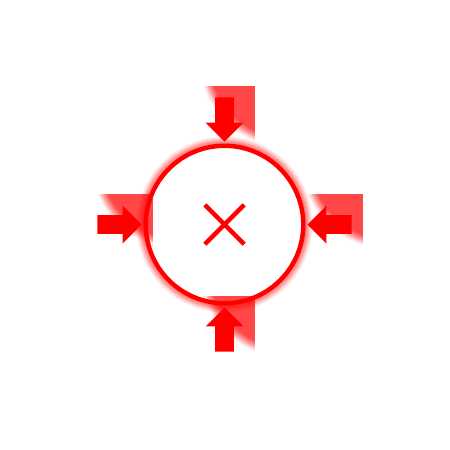
\begin{tikzpicture}[glow color=red]
 \pgfmathsetmacro{\myradius}{1+0.2*sin(\the\myangle)}
 \path[use as bounding box] (-2.5,-2.5) rectangle (2.5,2.5);
 \node[draw=red,ultra thick,circle,minimum size=2*\myradius cm,fill=white,
    glow,path picture={\draw (-0.25*\myradius,-0.25*\myradius) -- 
    (0.25*\myradius,0.25*\myradius)
    (-0.25*\myradius,0.25*\myradius) -- 
    (0.25*\myradius,-0.25*\myradius);},rotate=\the\myangle]{};
 \foreach \X in {0,90,180,270} 
 {\path (\X+\the\myangle:\myradius cm+0.05cm) node[anchor=east,marrow,rotate=\X+180+\the\myangle]{};}
\end{tikzpicture}
\end{frame}
\end{document}
